\renewcommand{\theauthor}{Matthias Franz}
\section{Datenbank}
\label{sec:datenbank}
In diesem Kapitel geht es um die Datenbank welche in dieser Arbeit erstellt worden ist. Es geht um den Aufbau der Datenbank, deren Funktion und wie diese mit den anderen Teilen des Projektes zusammenarbeitet.

\subsection{Funktion der Datenbank}
\label{sec:funktionDatenbank}
Die Datenbank speichert Benutzerdaten und Kalender der Benutzer. Die Daten dieser Datenbank bilden alle für dieses Projekt relevanten Teile einer iCal-Datei ab. Es werden nicht alle möglichen Eigenschaften einer iCal-Datei benötigt, da die Daten welche gespeichert werden ausreichen, um einen typischen Kalender welcher in Unternehmen verwendet wird abgebildet. Die Datenbank ermöglicht es, dass mehrere Benutzer mehrere Kalender haben und mehrere Benutzer auch die gleichen Kalender haben können. Benutzer sind in der Lage Kalender mit Terminen, To-Do Elementen und Alarmen zu speichern, weiters ermöglicht die Datenbank es die Zeitzone des Kalenders zu ändern.
\\
Die Daten werden dann vom Parser genommen und in eine funktionierende .ics-Datei umgewandelt. 

\subsection{Aufbau der Datenbank}
\label{sec:aufbauDatenbank}

\pagebreak
\begin{figure}[H]
	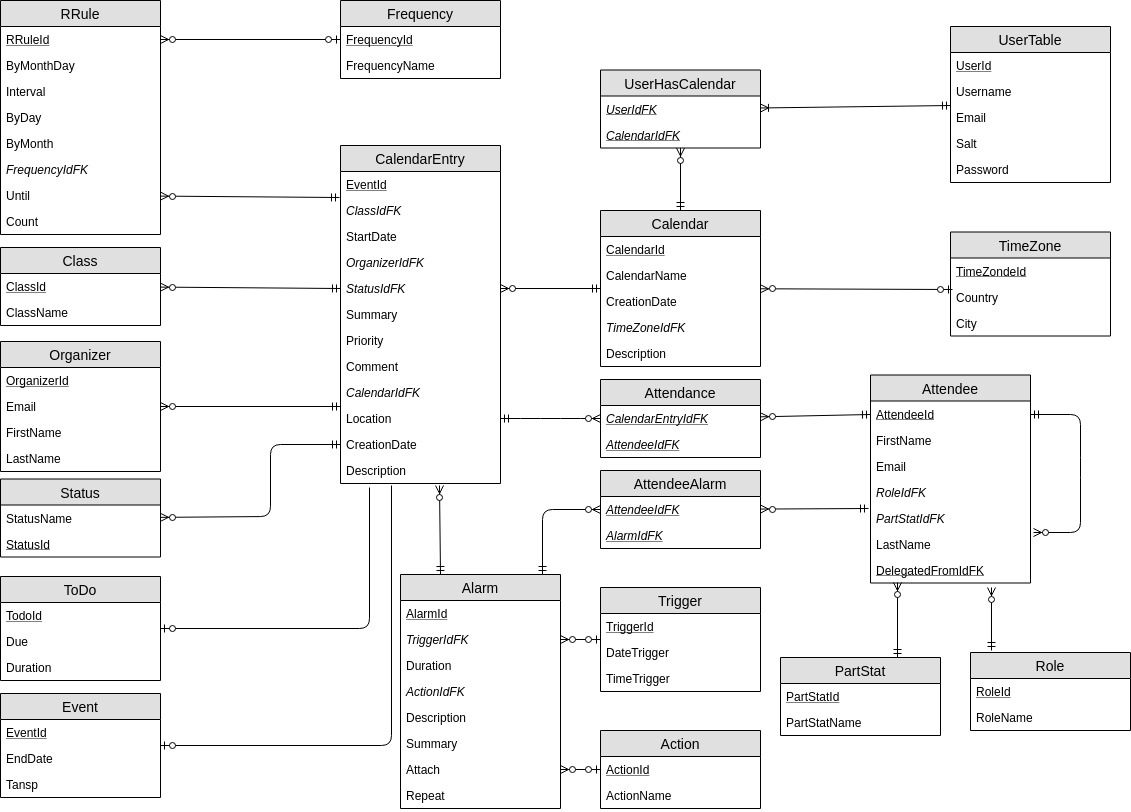
\includegraphics[angle=270,origin=c,width=\textwidth]{Datenbank_ER-Diagramm.jpg}
    \caption{ER-Diagramm}
    \label{fig:sprintBacklog}
\end{figure}
	
\pagebreak